\title{射影幾何自助餐} %標題
\author{張修展} %編輯這份講義的作者
\date{August 11, 2019}
\date{\today}%今天
\lfoot{Author:\theauthor}
\maketitle
\thispagestyle{fancy}
\raggedright
\rhead{模板}
\tableofcontents  % 生成目錄
%請在以下輸入內容

\setcounter{section}{-1}
\section{無窮遠炒麵線}
\pro
對於複平面上五點$z_{1}, z_{2}, z_{3},z_{4},z_{5}$,若\\
\[(z_{1},z_{2};z_{3},z_{4})=(z_{1},z_{2};z_{3},z_5)\]
則$z_{4}=z_{5}$\\


\section{表格}
\begin{tabular}[t]{|l|c|r|}
\hline%畫一條橫線
\diagbox{c}{r} & column2 & column3 \\
\hline%畫一條橫線
item1   & item2   & item3 \\
itemA   & itemB   & itemC \\
\hline
\end{tabular}

~\\%空行
~\\%空行


\section{方框}
\fbox{
  \parbox{\textwidth}{
想法:
容易發現$HA_{PH}C_{aH}C_{aP}, HB_{PH}C_{bH}C_{bP}, HC_{PH}C_{cH}C_{cP}$是平行四邊形,\\
欲構造共圓四點$UW_aW_bW_c$使$HA_{PH},HB_{PH},HC_{PH}$分別和$UW_a,UW_a,UW_a$\\
平行且長度比例相同即可證明命題\\

  }
}


\section{多欄位}
\begin{multicols}{2}
    \begin{enumerate}[label=(\roman*)]
    \item 取$P$為$\Delta ABC$垂心$H$
    \item {\color{blue}取$P$為$\Delta ABC$外心$O$}
    \item {\color[RGB]{0,255,200}取$Q$為$\Delta ABC$外心$O$}
    \item 取$P$為$\Delta ABC$外接圓上一點
    \item 取$P,Q$為同一點
    \item 取$Q$為$\Delta ABC$垂心$H$
    \item 當取$P$是定點時,$Q$滿足$H,A_3,B_3,C_3$四個共圓的軌跡不超過6次
    \end{enumerate}
\end{multicols}


\section{插入圖片}


\subsection{子圖並排}
\begin{figure}[H]
\centering  %图片全局居中
\subfigure[最左邊是小波]{
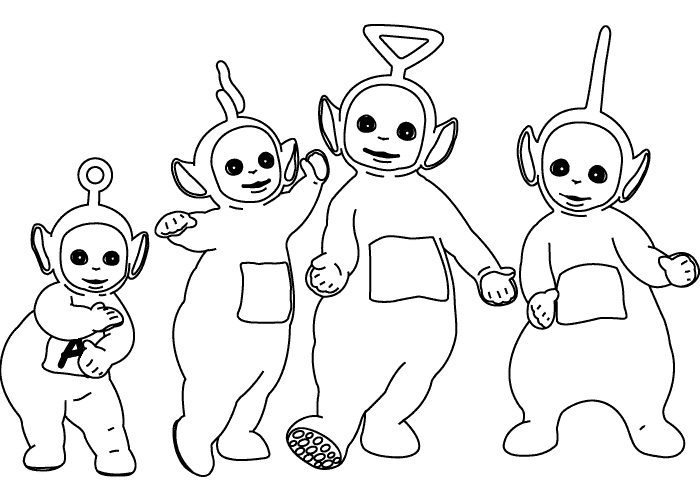
\includegraphics[width=0.3\textwidth]{a}}
\qquad\qquad\qquad
\subfigure[再來是拉拉]{
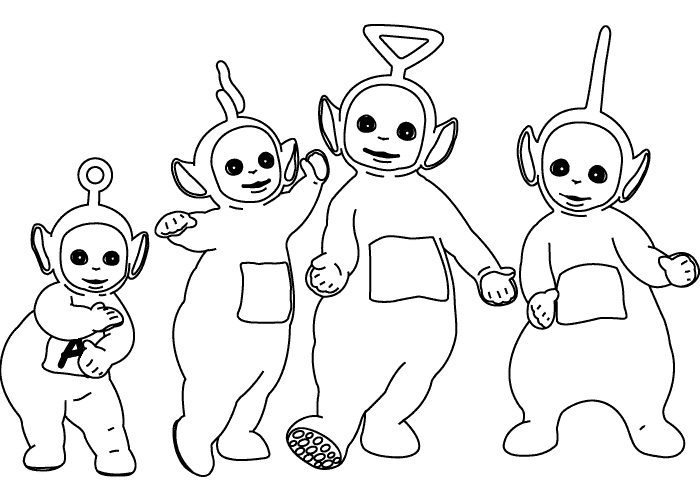
\includegraphics[width=0.3\textwidth]{a.png}}
\caption{小波和拉拉}
\label{fig:小波和拉拉}
\end{figure}

\subsection{圖片並排}
\begin{figure}[H]%與文字並排
  \centering %圖片全居中
  %並排幾個圖就要開幾個minipage
  \begin{minipage}[b]{0.4\textwidth} %minipage寬
    \centering %图片局部居中
    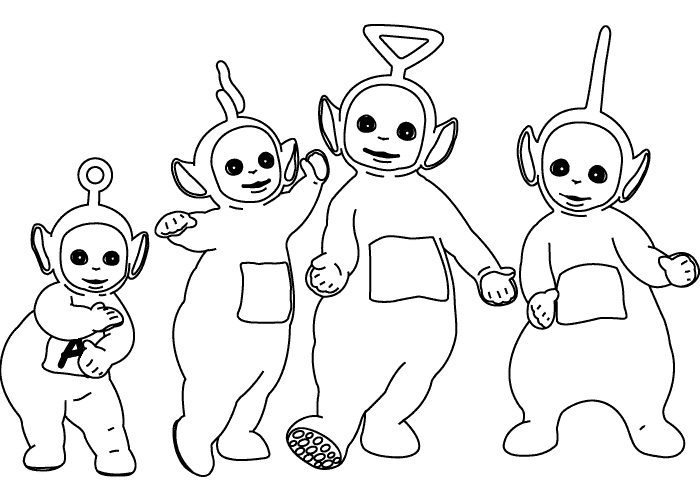
\includegraphics[width=0.8\textwidth]{a.png}
    \caption{最右邊是迪西}
    \label{fig:迪西}
  \end{minipage}
  \begin{minipage}[b]{0.4\textwidth} %minipage宽
    \centering %图片局部居中
    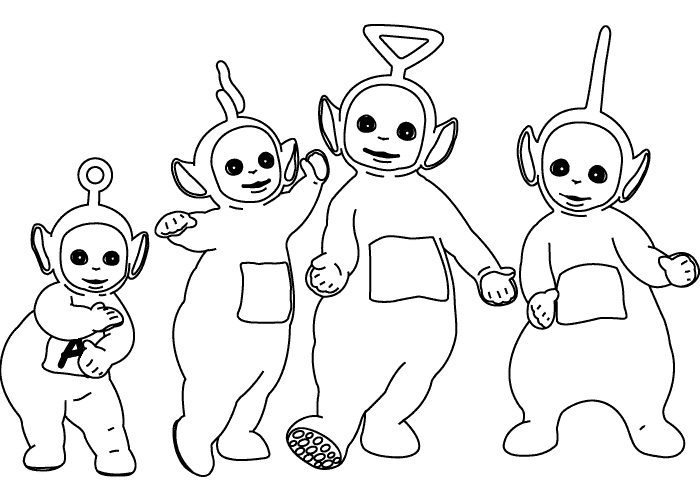
\includegraphics[width=0.8\textwidth]{a.png}
    \caption{再來是丁丁}
    \label{fig:丁丁}
  \end{minipage}
\end{figure}
所以
丁丁是\prettyref{fig:丁丁}
迪西是\prettyref{fig:迪西}
\section{Footnote}
我是原文\footnote{我是角標}
\newpage


\section*{My Chemical LaTeX}
\subsection*{一些語法}

\ce{2[AgCl2]-}\\
\begin{minipage}[b]{0.3\textwidth}
  \centering
  \chemfig{*6(-=-=-=)}\\
  \chemfig{*5(-----)}\\
\end{minipage}\\

\chemfig{*6(-=-=-=)}\\
\chemfig{*5(-----)}\\
\chemfig{A-B}\\
\chemfig{A=B}\\
\chemfig{A~B}\\
\chemfig{A>B}\\
\chemfig{A>:B}\\
\chemfig{A>|B}\\
\chemfig{C(-[1]1)(-[2]2)(-[3]3)(-[4]4)(-[5]5)(-[6]6)(-[7]7)(-[0]0)}
\ex 乙烯
\chemfig{C(-[3]H)(-[5]H)=C(-[1]H)(-[7]H)}
aaa
hi
